

 
The \code{lm} operator finds model coefficients. 
\index{P}{lm@\texttt{lm}}
\index{P}{Modeling!lm@\texttt{lm}}
\index{C}{coefficients!computing best fitting}
To illustrate,
here's a pair of statements that read in a data frame and fit a model
to it:
\begin{Schunk}
\begin{Sinput}
> swim = fetchData("swim100m.csv")
> mod = lm(time ~ year + sex, data=swim) 
\end{Sinput}
\end{Schunk}
The first argument to \code{lm} is a model design, the second is the data frame.

\datasetSwimming

The object  created by \code{lm} --- here given the name \code{mod} --- contains a variety of
information about the model.
To access the coefficients themselves, use the \code{coef}
\index{P}{coef@\texttt{coef}}
\index{P}{Modeling!coef@\texttt{coef}}
operator applied to the model:
\begin{Schunk}
\begin{Sinput}
> coef(mod)
\end{Sinput}
\begin{Soutput}
(Intercept)        year        sexM 
    555.717      -0.251      -9.798 
\end{Soutput}
\end{Schunk}

As shorthand to display the coefficients, just type the
name of the object that is storing the model:
\begin{Schunk}
\begin{Sinput}
> mod
\end{Sinput}
\begin{Soutput}
...
(Intercept)         year         sexM  
    555.717       -0.251       -9.798  
\end{Soutput}
\end{Schunk}

A more detailed report can be gotten with the \code{summary}
operator. 
\index{P}{summary@\texttt{summary}!for \texttt{lm}}
\index{P}{Modeling@regression report with \texttt{summary}}
\index{P}{Regression report with \texttt{summary}}
\index{C}{regression report!computing}
 This gives additional statistical information
that will be used in later chapters:
\begin{Schunk}
\begin{Sinput}
> summary(mod)
\end{Sinput}
\end{Schunk}
% latex table generated in R 2.13.0 by xtable 1.5-6 package
% Tue Aug 23 18:13:08 2011
\begin{tabular}{rrrrr}
  \hline
 & Estimate & Std. Error & t value & Pr($>$$|$t$|$) \\ 
  \hline
(Intercept) & 555.7168 & 33.7999 & 16.44 & 0.0000 \\ 
  year & -0.2515 & 0.0173 & -14.52 & 0.0000 \\ 
  sexM & -9.7980 & 1.0129 & -9.67 & 0.0000 \\ 
   \hline
\end{tabular}
\index{C}{model value!calculating}

From time to time in the exercises, you will be asked to calculate
model values ``by hand.''  This is accomplished by multiplying
the coefficients by the appropriate values and adding them up.  For
example, the model value for a male swimmer in 2010 would be:
\begin{Schunk}
\begin{Sinput}
> 555.7 - 0.2515*2010 - 9.798
\end{Sinput}
\begin{Soutput}
[1] 40.4
\end{Soutput}
\end{Schunk}
Notice that the ``value'' used to multiply the intercept is always 1,
and the ``value'' used for a categorical level is either 0 or 1
depending on whether there is a match with the level.  In this example,
since the swimmer in question was male, the value of \indicatorVar{sex}{M} is 1.
If the swimmer had been female, the value for
\indicatorVar{sex}{M} would have been 0.

When a model includes interaction terms, the interaction coefficients
need to be multiplied by all the values involved in the interaction.
For example, here is a model with an interaction between \VN{year} and
\VN{sex}:
\index{C}{interaction term!computing model values}
\begin{Schunk}
\begin{Sinput}
> mod2 = lm(time ~ year*sex, data=swim)
> coef(mod2)
\end{Sinput}
\begin{Soutput}
(Intercept)        year        sexM   year:sexM 
    697.301      -0.324    -302.464       0.150 
\end{Soutput}
\begin{Sinput}
> 697.3 - 0.3240*2010 - 302.5 + 0.1499*2010
\end{Sinput}
\begin{Soutput}
[1] 44.9
\end{Soutput}
\end{Schunk}
The \code{year:sexM} coefficient is being multiplied by the year
(2010) and the value of \indicatorVar{sex}{M}, which is 1 for this
male swimmer.

\subsubsection*{Other Useful Operators}

\begin{description}

\index{P}{cross@\texttt{cross}*}
\index{P}{Data!cross@\texttt{cross}*}
\index{C}{crossing categorical variables}
\index{C}{categorical variable!crossing}
\item[\function{cross}] will combine two categorical variables into a single
  variable.  For example, in the Current Population Survey data, the
  variable \VN{sex} has levels F and M, while the variable \VN{race}
  has levels W and NW.  Crossing the two variables combines them; the
  new variable has four levels: F.NW, M.NW, F.W, M.W:
\begin{Schunk}
\begin{Sinput}
> cps = fetchData("cps.csv")
> cross(cps$sex, cps$race)
\end{Sinput}
\end{Schunk}
\begin{Schunk}
\begin{Soutput}
 [1] M:W  M:W  F:W  F:W  M:W  F:W  F:W  M:W  M:W  F:W  M:W  M:W  M:W  M:W 
[15] M:W  M:W  M:W  M:NW M:NW M:W  F:NW M:NW
Levels: F:NW F:W M:NW M:W
... for 534 cases altogether ...
\end{Soutput}
\end{Schunk}

\index{P}{as.factor@\texttt{as.factor}}
\index{P}{Data!as.factor@\texttt{as.factor}}
\index{C}{categorical variable!from quantitative}
\index{C}{quantitative variable!to categorical}
\item[\function{as.factor}] will convert a quantitative variable to a categorical
  variable.  This is useful when a quantity like \VN{month} has been
  coded as a number, say 1 for January and 2 for February, etc.
  but you do not want models to treat it as such.

  To illustrate, consider two different models of the usage
  temperature versus month:
\begin{Schunk}
\begin{Sinput}
> utils = fetchData("utilities.csv")
> mod1 = lm(temp ~ month, data=utils)
> mod2 = lm(temp ~ as.factor(month), data=utils)
\end{Sinput}
\end{Schunk}

\datasetUtilities
Here are the graphs of those models:

\begin{Schunk}
\begin{Sinput}
> xyplot(temp + fitted(mod1) ~ month, data=utils)
\end{Sinput}
\end{Schunk}
\includegraphics{Figures/formulas-util-mod1}

\begin{Schunk}
\begin{Sinput}
> xyplot( temp + fitted(mod2) ~ month, data=utils )
\end{Sinput}
\end{Schunk}
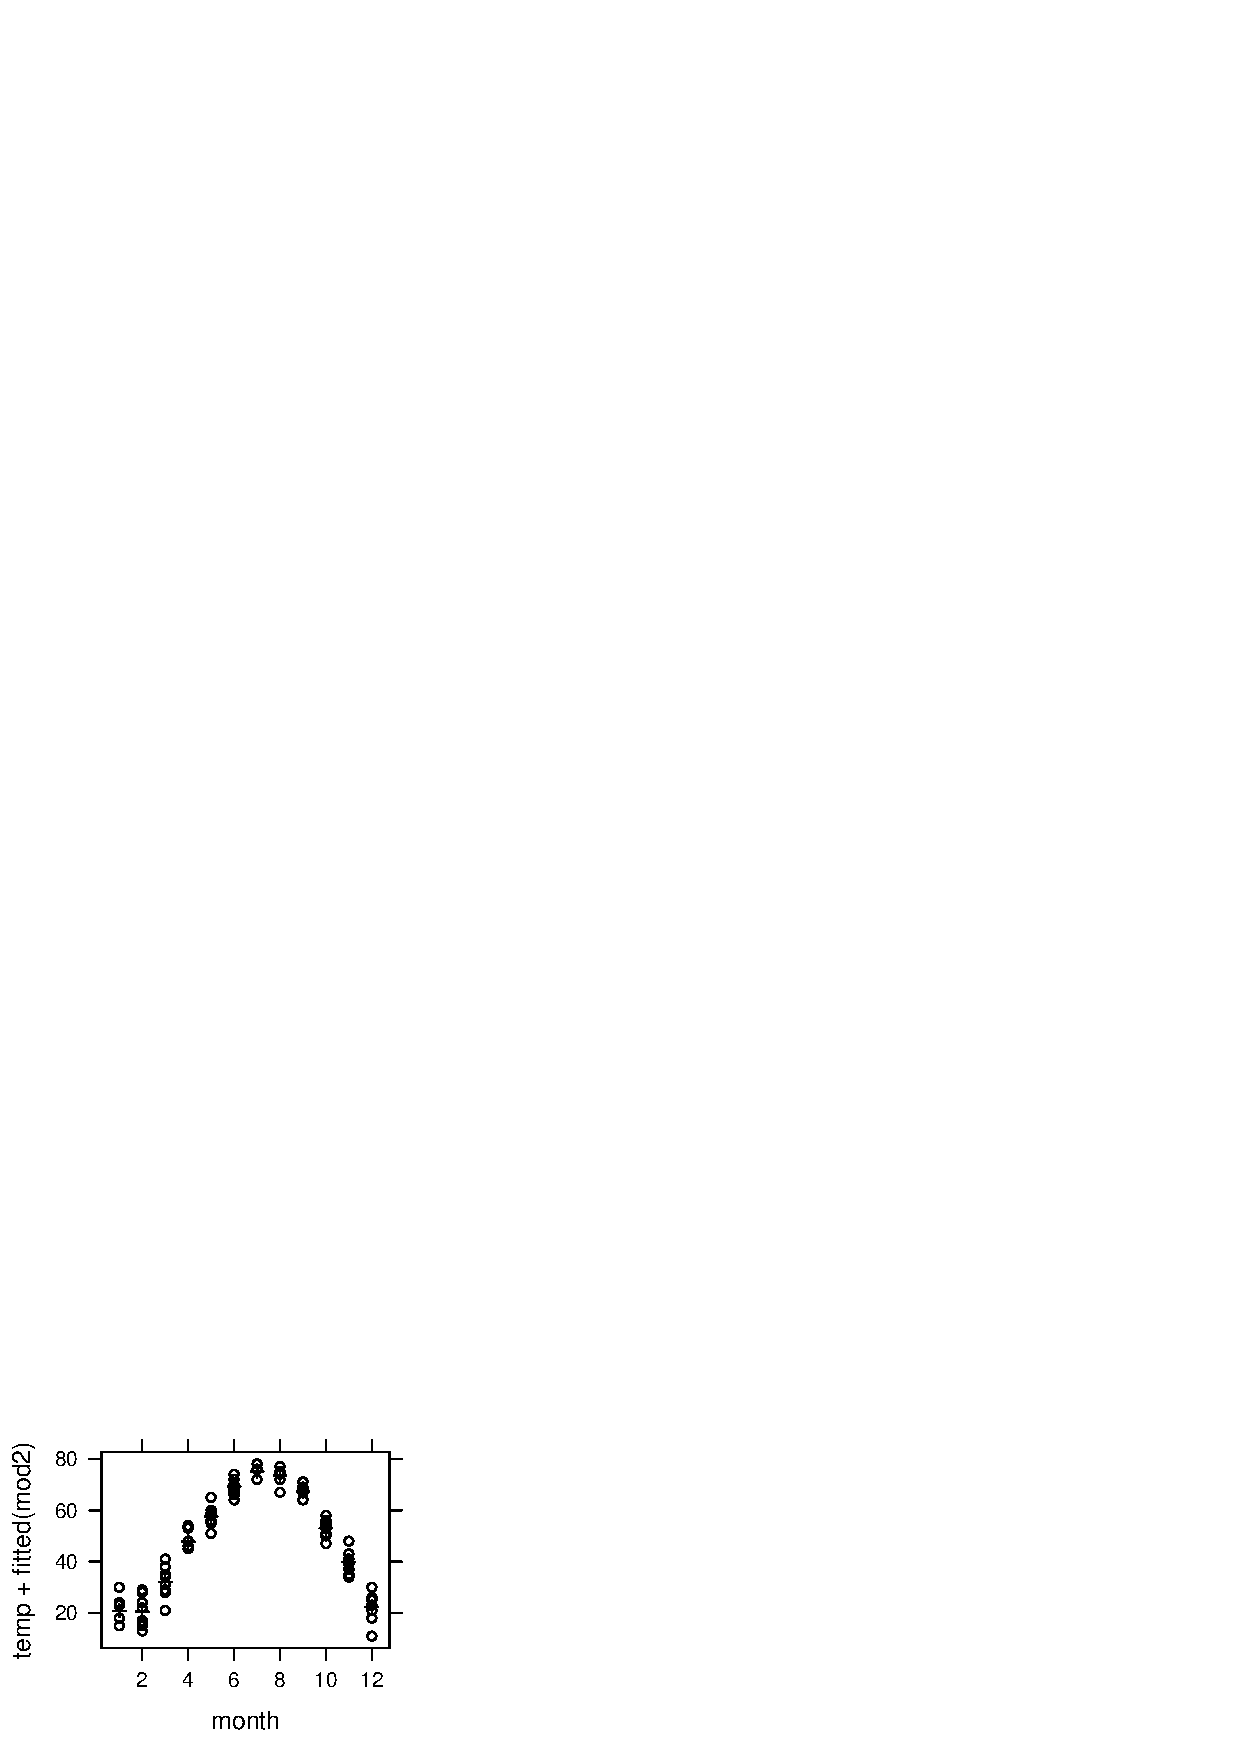
\includegraphics{Figures/formulas-util-mod2}



\begin{comment}
utils = read.csv("/users/kaplan/kaplanfiles/sbook/datasets/utilities.csv")
mod1 = lm( temp ~ month, data=utils)
xyplot( temp ~ month, data=utils, main="Model 1")
trellis.focus()
x = seq(1,12)
y = 39.04 + 1.63*x
llines(x,y,col='red',lwd=3)
trellis.unfocus()
\end{comment}

\begin{comment}
mod2 = lm( temp ~ as.factor(month)-1, data=utils)
x = 1:12
y = as.numeric( coefficients(mod2))
xyplot( temp ~ month, data=utils, main="Model 2")
trellis.focus()
llines(  x,y, lwd=3, col='red')
trellis.unfocus()
\end{comment}

In the first model, month is treated quantitatively, so the model term
\VN{month} produces a straight-line relationship that does not
correspond well to the data.

In the second model, month is treated categorically, allowing a more
complicated model relationship.

% \item[abbreviate] shortens the names of factors

\end{description}
